\documentclass[miniframe]{lbpbeamer}
%\documentclass[handout]{lbpbeamer}
%%%%%%%%%%%%% option de la classe lbpbeamer.cls
% toutes les options standards de la classe beamer
% le type d'en-tete pour l'appel des sections : 
%  - default : currentsection | currentsubsection
%  - miniframe : sections + puces
%  - tree : sections + currentsubsection
%  - split : sections + subsections
%%%%%%%%%%%%%%%%%%%%%%%%%%%%%%%%%%%%%%%%%%%%%%%%%%

%%%%%%%%%%%%% appel des packages
\usepackage[english,french]{babel}
\usepackage{epsfig}
\usepackage[T1]{fontenc}
\usepackage[utf8]{inputenc}
\usepackage{lmodern} 
\usepackage{times}
\usepackage{multirow}
\usepackage{animate}
\usepackage{hyperref}
\usepackage{movie15}
\usepackage{wasysym}
\usepackage[squaren, Gray, cdot]{SIunits}
\usepackage{tikz}
\usetikzlibrary{calc,trees,positioning,arrows,chains,shapes.geometric,%
	decorations.pathreplacing,decorations.pathmorphing,shapes,%
matrix,shapes.symbols,plotmarks,decorations.markings,shadows}

\usepackage{tabularx}
\newcolumntype{L}[1]{>{\raggedright\let\newline\\\arraybackslash\hspace{0pt}}m{#1}}
\newcolumntype{C}[1]{>{\centering\let\newline\\\arraybackslash\hspace{0pt}}m{#1}}
\newcolumntype{R}[1]{>{\raggedleft\let\newline\\\arraybackslash\hspace{0pt}}m{#1}}

\newcommand{\backupbegin}{
	\newcounter{framenumberappendix}
	\setcounter{framenumberappendix}{\value{framenumber}}
}
\newcommand{\backupend}{
	\addtocounter{framenumberappendix}{-\value{framenumber}}
	\addtocounter{framenumber}{\value{framenumberappendix}} 
}

%\usepackage{enumitem}

%%%%%%%%%%%%%%%%%%%%%%%%%%%%%%%%%%%%%%%%%%%%%%%%%%
%\newlist{fleche}{itemize}{1}
%\setlist[fleche]{label=$\rightarrow$,font=\color{blue}}


%\newcommand{\smiley}{\tikz[baseline=-0.75ex,black]{
%		    \draw circle (2mm);
%			\node[fill,circle,inner sep=0.5pt] (left eye) at (135:0.8mm) {};
%			\node[fill,circle,inner sep=0.5pt] (right eye) at (45:0.8mm) {};
%			\draw (-145:0.9mm) arc (-120:-60:1.5mm);
%			    }
%			}

\newcommand{\orto}{^{\circ}}

%%%%%%%%%%%%% appel du plan a chaque subsection
%% en 1 colonne

%\AtBeginSection[]{
%	\frame{%<handout:0>{
%	\frametitle{Plan}
%  \begin{columns}[t]
%  \begin{column}{0.5\linewidth}
%  \tableofcontents[sections={1-3}, currentsection,subsectionstyle=show/show/shaded]
%  \end{column}
%  \begin{column}{0.5\linewidth}
%  \tableofcontents[sections={4-6}, currentsection,subsectionstyle=show/show/shaded]
%  \end{column}
%  \end{columns}
%  }
%}

%% ou en 2 colonnes s'il y a trop de sections
    
%\AtBeginSubsection[]{
%	\frame{%<handout:0>{
%	\frametitle{Summary}
%  \begin{columns}[t]
%  \begin{column}{0.5\linewidth}
%  \tableofcontents[sections={1-6},currentsection, subsectionstyle=show/shaded/hide]
%  \end{column}
%  \begin{column}{0.5\linewidth}
%  \tableofcontents[sections={7-12},currentsection,subsectionstyle=show/shaded/hide]
%  \end{column}
%  \end{columns}
%  }
%}	
%%%%%%%%%%%%%%%%%%%%%%%%%%%%%%%%%%%%%%%%%%%%%%%%%%	

%%%%%%%%%%%%% Pour supprimer les symboles de navigation
\setbeamertemplate{navigation symbols}{}
%%%%%%%%%%%%%%%%%%%%%%%%%%%%%%%%%%%%%%%%%%%%%%%%%%

%%%%%%%%%%%%% Personnalisation des theoremes
\newtheorem{theoreme}{Th\'eor\`eme}
\newtheorem{preuve}{D\'emonstration}
\newtheorem{define}{D\'efinition}
%%%%%%%%%%%%%%%%%%%%%%%%%%%%%%%%%%%%%%%%%%%%%%%%%%	
		
%%%%%%%%%%%%% Infos personnelles au document	
\title[Anecdote intéressante]{Anecdote intéressante}
\subtitle{Ou \og{}pourquoi que c'est important de faire attention au codage de l'information\fg{}}
\author[Fiack]{Laurent Fiack}
%\email{}
\institute[Lycée Blaise Pascal]{Lycée Blaise Pascal}
\date[\today]{\today}
\logo{}
%%%%%%%%%%%%%%%%%%%%%%%%%%%%%%%%%%%%%%%%%%%%%%%%%%

\newcommand{\figpath}{figures/}

\usepackage{scrextend}

\begin{document}

%%%%%%%%%%%%% Background des slides	
\usebackgroundtemplate{}
%% cet option permet d'ins\'erer une image en fond-ecran
%% la commande \usebackgroundtemplate{} permet de
%% supprimer le fond a partir du moment ou il est 
%% appele
%%%%%%%%%%%%%%%%%%%%%%%%%%%%%%%%%%%%%%%%%%%%%%%%%%	

%%%%%%%%%%%%% frame title
\frame{\titlepage}
\usebackgroundtemplate{}
\logo{}
%\logoheader{taille}{emplacement-image}
%% on supprime les logos des autres frames		
%%%%%%%%%%%%%%%%%%%%%%%%%%%%%%%%%%%%%%%%%%%%%%%%%%
\section[Vol 501]{Ariane 5 : le vol 501}
\subsection[Vol 501]{Ariane 5 : le vol 501}

\frame{
	\centering
	\Huge
	Inspiré de faits réels
}

\frame{
	\frametitle{Ariane 5 : Vol 501}

	\begin{minipage}[b]{0.48\linewidth}
		\begin{itemize}
				\onslide<1->{
				\item 4 juin 1996
				}
				\onslide<2->{
				\item ESA (European Space Agency)
				}
				\onslide<3->{
				\item 1er vol Ariane 5
				}
				\onslide<5->{
				\item Ariane 4 très fiable
				}
				\onslide<6->{
					\vspace{1em}
					\begin{center}
						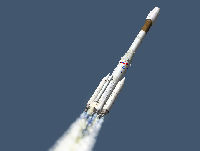
\includegraphics[width=.6\linewidth]{./figures/ariane4.png}
					\end{center}
				}
		\end{itemize}
	\end{minipage}
	\hfill
	\begin{minipage}[b]{0.48\linewidth}
		\begin{center}
		\onslide<4->{
			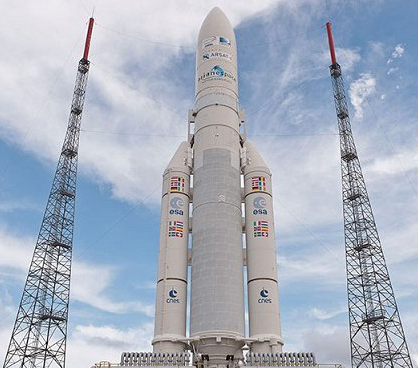
\includegraphics[width=.9\linewidth]{./figures/ariane5.png}
		}
		\end{center}
		\begin{itemize}
			\onslide<7->{
			\item 4 satellites = \$370M
			}
			\onslide<8->{
			\item 36,7 secondes plus tard...
			}
		\end{itemize}
	\end{minipage}
}

\frame{
	\frametitle{36,7 secondes ; 4000 mètres}
	\begin{center}
		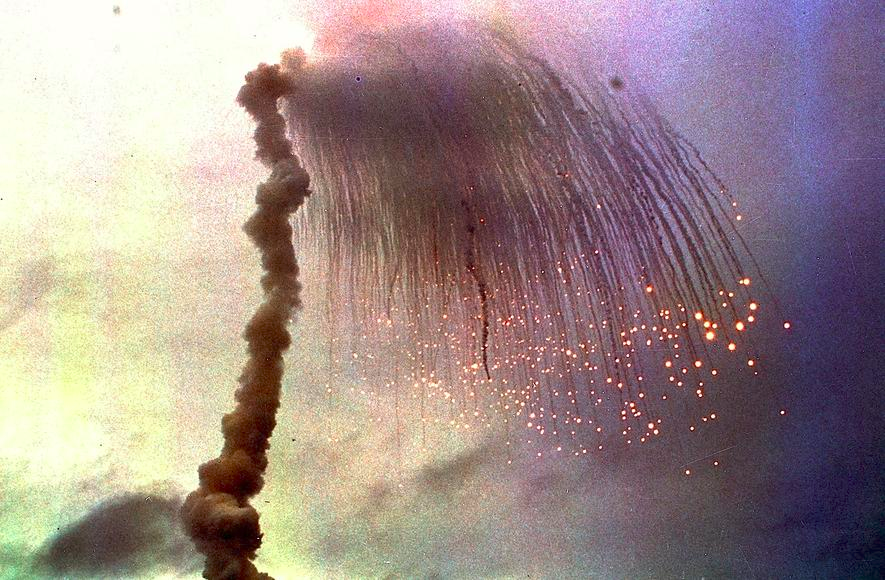
\includegraphics[width=.9\linewidth]{./figures/ariane5_explosion.png}
	\end{center}
}

\frame{
	\frametitle{Que s'est-il donc passé ?}
	\begin{minipage}[b]{0.48\linewidth}
		\begin{itemize}
			\onslide<1->{
			\item Un peu de mécanique orbitale\\
			}
			\begin{center}
				\begin{tikzpicture}[scale=1]
					\onslide<2->{
						\draw (0,0) circle (1.5);
						\draw (0,0) node{Terre};
					}
					\onslide<3>{
						\draw (0,1.5) -- (0,1.7);
						\draw [fill=black] (0,1.7) circle (0.05);
					}
					\onslide<4>{
						\draw (0,1.5) -- (0,2);
						\draw [fill=black] (0,2) circle (0.05);
					}
					\onslide<5>{
						\draw (0,1.5) -- (0,2.5);
						\draw [fill=black] (0,2.5) circle (0.05);
					}
					\onslide<6->{
%						\draw (0,1.5) parabola (1.414,1.414);
						\draw (0,1.5) ..controls (0.2,1.9) and (1,1.732) .. (1.414,1.414);
						\draw [fill=black] (1.414,1.414) circle (0.05);
					}
					\onslide<7->{
						\draw [dashed] (0,0) circle (2);
					}
				\end{tikzpicture}	
			\end{center}
		\end{itemize}
	\end{minipage}
	\hfill
	\begin{minipage}[b]{0.48\linewidth}
		\begin{itemize}
			\onslide<8->{
			\item Capteur d'accélération horizontale
			}
			\onslide<9->{
			\item Valeur max = 60, rentre sur 1 octet
			}
			\onslide<10->{
			\item Ariane 5 plus puissante
			\item Accélération horiz. plus forte
			}
			\onslide<11->{
			\item Valeur max = 300
				\vspace{2em}
			\item \textbf{Que se passe-t-il?}
			}
		\end{itemize}
	\end{minipage}
}

\frame{
	\frametitle{Conclusion}
	\onslide<1->{
		Au final, cette \og{}boulette\fg{} a couté 370 millions de dollars,
	}
	\onslide<2->{
		plus le prix du lanceur,
	}
	\onslide<3->{
		plus la perte de confiance de la part des clients de l'ESA 
	}
	\onslide<4->{
		(ce qui a probablement coûté beaucoup plus cher au final).\\
	}
	\vspace{1em}
	\onslide<5->{
		Évidemment, cette boulette aurait pu être évitée par une simple simulation ou un vol d'essai.\\
	}
	\vspace{1em}
	\onslide<6->{
		Mais par cet exemple un peu extrême, on voit concrètement l'intérêt de se poser des questions de codage et de représentation de l'information.
	}
}

\end{document}
